%!TEX root = ../main.tex

\section{Data Rate}\label{sec:data_rate}
This section will explore the amount of data that can be expected from a data producer connected to the system.
Many of these parameters of interest pose different requirements in terms of the desired sample rate as well as the size of each sample.
A temperature sensor, for instance, does not require nearly the same sampling frequency as an accelerometer.
Due to these differences the data rate expected from one data producer may differ wildly from another.
In order to provide a safe estimate, the expected data rate is calculated using a worst case sensor.
That is, the type of sensor which sets the highest requirements in terms of sampling frequency as well as data size.
Again, it is not possible to foresee every application that may be developed in the future.
Despite of this the IMU chosen for this project, see section~\ref{sec:imu}, is considered as the worst-case.
It is is a 9-axis sensor that provides data at a rate up to 300 Hz at 32 bit floating point precision.
This would result in a data rate of:
\martin{Recalculate this equation}

$$400\cdot32\cdot9=115.2\,\text{Kb/s}$$

As previously mentioned, this is the assumed worst case for the system.
As such there may be only a few data producers providing data at this rate.
Most other producers will provide only limited data in relation to the IMU, either due to a much lower sampling frequency or an overall smaller data size.
A GPS generally provides an update only at a few \si{\hertz}. 
An encoder, while it may have a reasonably high sampling rate, it is most likely not close to 32 bit resolution.
\\~\\
Assuming five sensors running at the assumed worst case rate and ten running at half that rate, the resulting data rate will be 1.15 Mb/s.

% \subsection{Data Logging}
% \todo[inline]{Mikkel: Should maybe change name?}
% A feature will be data logging. 
% Any data could be put into the log, although some signals can be logged at significantly higher rates than others
% If all data is recorded at the fastest rate, this could present a storage problem.
% This challenge will be analyzed here.

% \subsubsection{Sample Rate}
% Datalogging should be useful for working with an inverter as was the case on the first semester.
% Likely it would be interesting to log the phase-current to the motor at high enough rate to accurately depict their sinusoidal short term average.
% The ripple current or voltage at the motor terminals should be measured in the lab, as this requires a high sample rate, and more control than offered on the test track.
% This data logging would be useful for recording current in the motor as the go kart is driving.
% Additionally it would be relevant to record the encoder output, and possibly the DC voltage at the input of the inverter and the duty for each phase.
% Only the currents are bound to change rapidly, and as such they determine the minimum acceptable sample rate.
% By looking at the maximum frequency of the motor and the most extreme rate of change permissible by the armature inductance, it is possible to set a sample rate for the log file.\\

% According to the manufacturer of the motor, the maximum rotational velocity is 5000 RPM.
% With four pole pairs, this comes to a maximum sinusoidal frequency of 333 Hz. 
% It is not necessary to record at a rate significantly larger than the Nyquist limit in order to adequately record the sinusoidal.
% Simulations show, that by using Clark-Park transformation, interpolation and then the inverse Clarke-Park transformation, there is nearly no difference between a low sample rate of $1\si{\kilo\hertz}$, and a higher sample rate of $3.3\si{\kilo\hertz}$, as shown below.

% \begin{figure}
% 	\centering
% 	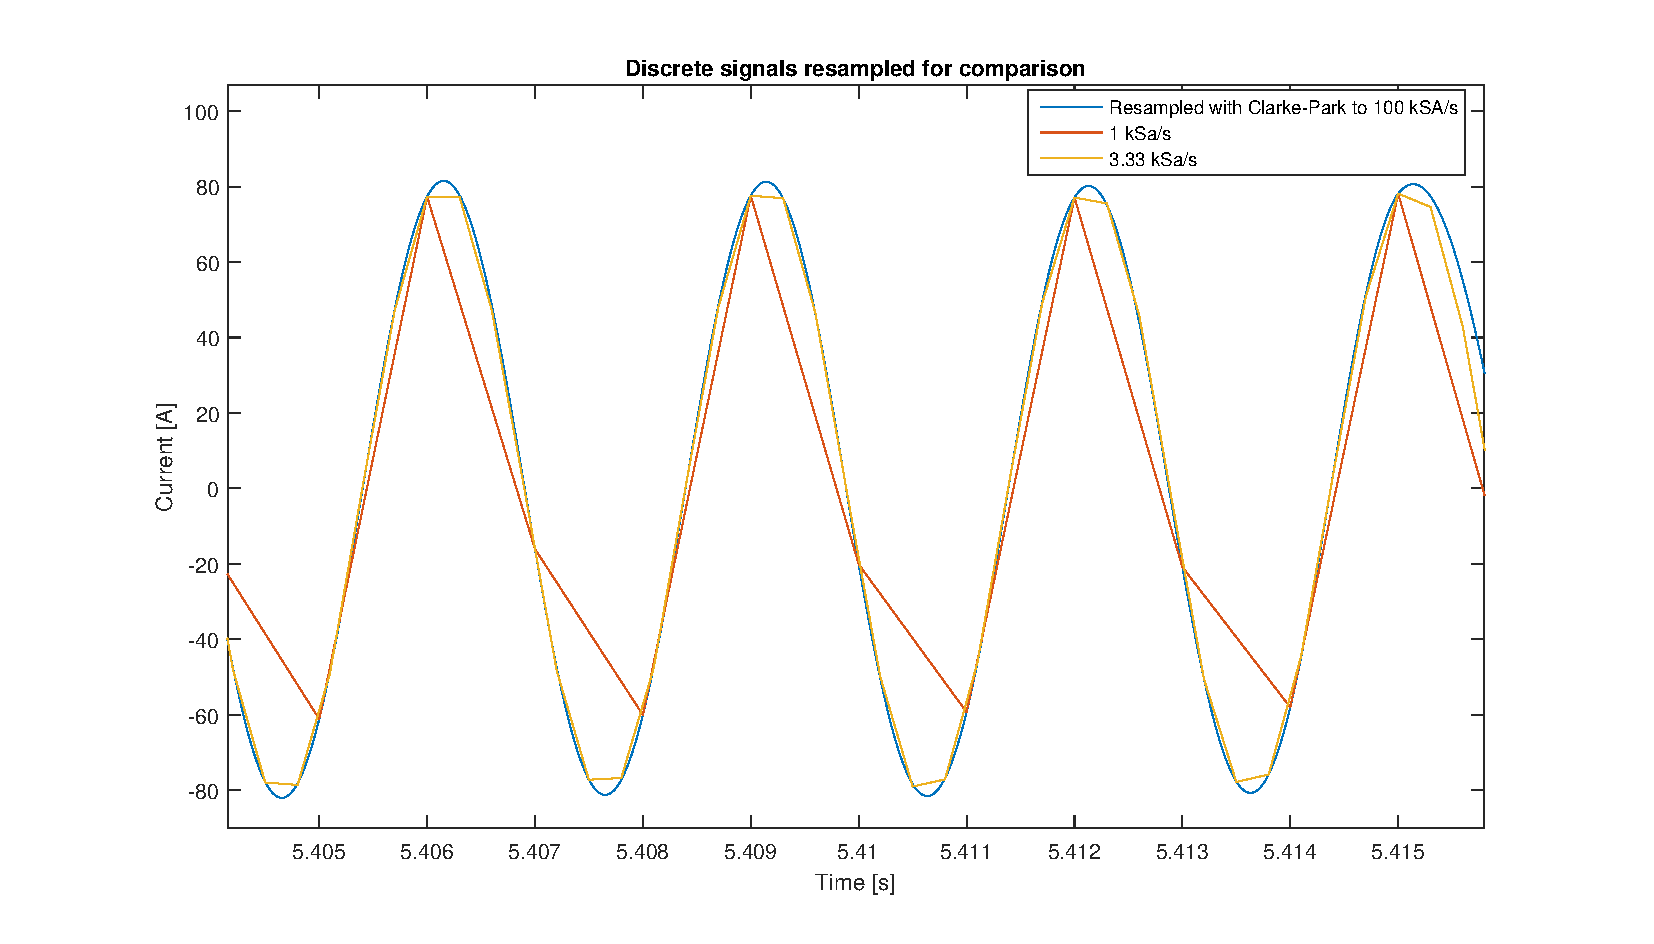
\includegraphics[width = 0.9\linewidth]{graphics/Clarke-park_resampled}	
% 	\caption{Comparison of data recorded at 1 kSa/s and 3.33 kSa/s, against 100 kSa/s resampled using Clarke-Park}
% 	\label{fig:Clarke-park_resampled}
% \end{figure}

% The resampled data from the 1 kSa/s and 3.3 kSa/s (orange and purple respectively on figure\ref{fig:Clarke-park_resampled}) are almost identical.
% However, there is a small visible difference around the time 5.527 s, likely due to the limited precision of the encoder.
% This also doesn't take into account any disturbance or noise, which could make it hard to reconstruct the signals with lower sample rates.\\

% Additionally, the Matlab function, resample, produces nicely filtered vectors with smaller time steps, so it is possible to use a low sample rate for time invariant signals.\\
% Another way to look at this is to calculate the maximum change in current from one sample to another.
% This is determined by the inductance of the motor, which is $600 \si{\micro \henry}$ \todo[inline]{when one half bridge is high, and the two others are low, it's one armature inductance of 400 uH in series with two parallel armature inductances}, and the maximum voltage across it, which is $V_{BAT}=52.8 \si{\volt}$. 
% At a sample rate of 3.33 kSa/s, this results in a theoretical maximum step of $264\si{\ampere}$.
% A sample rate lower than this, would make it hard to properly record such sudden steps.

% \subsubsection{Data Type}
% When the sample rate is known, it is possible to get an estimate of how much storage space would be needed. 
% It would be easiest, and most useful, to record using simple comma separated files, but these tend to take up more space than necessary.
% The analog input to the Zybo are 12 bit, which means, that full precision of these would be possible with 4 digits, and often a decimal point and potentially a negative sign.
% Including the horizontal separator, this comes to 6.5 bytes per point.\\

% An example of recording could include time, two currents, a voltage and the encoder output, as displayed below
% \begin{lstlisting}
% Time	Ia	Ib	V	Encoder
% 1.0000	052.3	-278.1	52.56	16
% 1.0003	057.7	-280.4	52.54	17
% \end{lstlisting}
% That brings each line length to 32 bytes (8 bytes for time, 5.5 for the three analog, 3 bytes for encoder, 5 for separators).
% At a sample rate of 3.33 kSa/s, this comes to 6.1MB per minute. 
% With the current SD cards having 4 GB of free un-partitioned space, this gives up to 11 hours of recording time.\\

% Alternately, it is possible to invent a file structure, that allows several arrays of with different data types.
% By storing numbers in binary files instead of text, it is possible to reduce the space requirements to a third (2 bytes per analog, 4 bytes per timestamp (allowing up to 49 days of ms), and 1 byte for encoder).
% This however will reduce the readability greatly, and include the workload, as one will need to write code both for encoding and decoding the file. \\

% Since this is out of the scope of this project, and the sample rate isn't larger than it is, logging in standard ASCII will suffice.
% Likely, different sample rates will be recorded to different log files